\documentclass[a4paper]{article}
\usepackage{tikz}
\usepackage{geometry}
\usepackage{graphicx}
\usepackage{natbib}
\usepackage{amsmath}
\usepackage{amssymb}
\usepackage{amsthm}
\usepackage{paralist}
\usepackage{epstopdf}
\usepackage{tabularx}
\usepackage{longtable}
\usepackage{multirow}
\usepackage{multicol}
\usepackage[hidelinks]{hyperref}
\usepackage{fancyvrb}
\usepackage{algorithm}
\usepackage{algorithmic}
\usepackage{float}
\usepackage{paralist}
%\usepackage[svgname]{xcolor}
\usepackage{enumerate}
\usepackage{array}
\usepackage{times}
\usepackage{url}
\usepackage{fancyhdr}
\usepackage{comment}
\usepackage{environ}
\usepackage{times}
\usepackage{textcomp}
\usepackage{caption}
\usepackage{bbm}


\urlstyle{rm}

\setlength\parindent{0pt} % Removes all indentation from paragraphs
\theoremstyle{definition}
\newtheorem{definition}{Definition}[]
\newtheorem{conjecture}{Conjecture}[]
\newtheorem{example}{Example}[]
\newtheorem{theorem}{Theorem}[]
\newtheorem{lemma}{Lemma}
\newtheorem{proposition}{Proposition}
\newtheorem{corollary}{Corollary}

\floatname{algorithm}{Procedure}
\renewcommand{\algorithmicrequire}{\textbf{Input:}}
\renewcommand{\algorithmicensure}{\textbf{Output:}}
\newcommand{\abs}[1]{\lvert#1\rvert}
\newcommand{\norm}[1]{\lVert#1\rVert}
\newcommand{\RR}{\mathbb{R}}
\newcommand{\CC}{\mathbb{C}}
\newcommand{\Nat}{\mathbb{N}}
\newcommand{\br}[1]{\{#1\}}
\DeclareMathOperator*{\argmin}{arg\,min}
\DeclareMathOperator*{\argmax}{arg\,max}
\renewcommand{\qedsymbol}{$\blacksquare$}

\definecolor{dkgreen}{rgb}{0,0.6,0}
\definecolor{gray}{rgb}{0.5,0.5,0.5}
\definecolor{mauve}{rgb}{0.58,0,0.82}

\definecolor{C0}{HTML}{1F77B4}
\definecolor{C1}{HTML}{FF7F0E}
\definecolor{C2}{HTML}{2ca02c}
\definecolor{C3}{HTML}{d62728}
\definecolor{C4}{HTML}{9467bd}
\definecolor{C5}{HTML}{8c564b}
\definecolor{C6}{HTML}{e377c2}
\definecolor{C7}{HTML}{7F7F7F}
\definecolor{C8}{HTML}{bcbd22}
\definecolor{C9}{HTML}{17BECF}

\newcommand{\Var}{\mathrm{Var}}
\newcommand{\Cov}{\mathrm{Cov}}
\newcommand{\sgn}{\mathrm{sgn}}

\newcommand{\vc}[1]{\boldsymbol{#1}}
\newcommand{\xv}{\vc{x}}
\newcommand{\Sigmav}{\vc{\Sigma}}
\newcommand{\alphav}{\vc{\alpha}}
\newcommand{\muv}{\vc{\mu}}

\newcommand{\red}[1]{\textcolor{red}{#1}}

\def\x{\mathbf x}
\def\y{\mathbf y}
\def\w{\mathbf w}
\def\v{\mathbf v}
\def\E{\mathbb E}
\def\R{\mathbb R}
\def\V{\mathbb V}
\def\ind{\mathbbm 1}

% TO SHOW SOLUTIONS, include following (else comment out):
\newenvironment{soln}{
    \leavevmode\color{blue}\ignorespaces
}{}


\hypersetup{
%    colorlinks,
    linkcolor={red!50!black},
    citecolor={blue!50!black},
    urlcolor={blue!80!black}
}

\geometry{
  top=1in,            % <-- you want to adjust this
  inner=1in,
  outer=1in,
  bottom=1in,
  headheight=3em,       % <-- and this
  headsep=2em,          % <-- and this
  footskip=3em,
}


\pagestyle{fancyplain}
\lhead{\fancyplain{}{Homework 7}}
\rhead{\fancyplain{}{CS 760 Machine Learning}}
\cfoot{\thepage}

\title{\textsc{Homework 7}} % Title

%%% NOTE:  Replace 'NAME HERE' etc., and delete any "\red{}" wrappers (so it won't show up as red)

\author{
\red{$>>$NAME HERE$<<$} \\
\red{$>>$ID HERE$<<$}\\
} 

\date{}

\begin{document}

\maketitle 

\textbf{Instructions:}
Use this latex file as a template to develop your homework. Please submit a single pdf to Canvas. Late submissions may not be accepted. You can choose any programming language (i.e. python, R, or MATLAB). Please check Piazza for updates about the homework.
\vspace{0.1in}

\section{Kernel SVM [15 pts]}
Consider the following kernel function defined over $z,z'\in Z$:
\begin{align*}
k(z,z') =
\begin{cases}
1 & \text{~if~} z=z', \\
0 & \text{~otherwise.}
\end{cases}
\end{align*}
\begin{enumerate}
\item (5 pts) Prove that for any integer $m>0$, any $z_1, \ldots, z_m \in Z$, the $m \times m$ kernel matrix $K=[K_{ij}]$ is positive semi-definite, where $K_{ij}=k(z_i, z_j)$ for $i,j=\{1\ldots m\}$. (Let us assume that for $i \neq j$, we have $z_i \neq z_j$.)

\item (5 pts) Given a training set $(z_1, y_1), \ldots, (z_n, y_n)$ with binary labels, the dual SVM problem with the above kernel $k$ will have parameters $\alpha_1, \ldots, \alpha_n, b \in \R$.  (Assume that for $i \neq j$, we have $z_i \neq z_j$.) The predictor for input $z$ takes the form
$$f(z) = \sum_{i=1}^n \alpha_i y_i k(z_i, z) + b.$$
Recall the label prediction is $\sgn(f(z))$.
Prove that there exists $\alpha_1, \ldots, \alpha_n, b$ such that $f$ correctly separates the training set.
In other words, $k$ induces a feature space rich enough such that in it any training set can be linearly separated.

\item (5 pts) How does that $f$ predict input $z$ that is not in the training set?

\end{enumerate}

Comment: One useful property of kernel functions is that the input space $Z$ does not need to be a vector space; in other words, $z$ does not need to be a feature vector.  For all we know, $Z$ can be turkeys in the world.  As long as we can compute $k(z,z')$, kernel SVM works on turkeys.

\section{Game of Classifiers [50 pts]}
 \subsection{Implementation}
  Implement the following models in choice of your programming language. Include slack variables in SVM implementation if needed. You can use autograd features of pytorch, tensorflow etc. or derive gradients on your own. (But don't use inbuilt models for SVM, Kernel SVM and Logistic Regression from libraries)
  
  \begin{itemize}
      \item Implement Linear SVM (without kernels). 
      \item Implement Kernel SVM, with options for linear, rbf and polynomial kernels. You should keep the kernel parameters tunable (e.g. don't fix the degree of polynomial kernels but keep it as a variable and play with different values of it. Is Linear SVM a special case of Kernel SVMs?
      \item Implement Logistic Regression with and without kernels (use same kernel as Question 1).
      
  \end{itemize}
 \subsection{Evaluation on Synthetic Dataset}
 \subsubsection{Synthetic Dataset-1 (20 pts)}
 Generate 2-D dataset as following, \\
 Let $\mu=2.5$ and $I_2$ be the $2\times2$ identity matrix. Generate points for the positive and negative classes respectively from $\mathcal{N}([\mu,0],I_2)$, and $\mathcal{N}([-\mu,0],I_2)$. For each class generate 750 points, (1500 in total). Randomly create train, validation and test splits of size 1000, 250, 250 points respectively. Do the following with this dataset:
 \begin{itemize}
     \item (5 pts) Train your Linear SVM, Logistic Regression models and report decision boundaries, test accuracies. 
     \item (5 pts) Show decision boundaries with K-NN and Naive Bayes Classifiers. ( You can use library implementations or implement from scratch. Figure out the hyper-parameters using the validation set.) 
     \item (5 pts) Repeat the process by varying $\mu$ from 1.0 to 2.4 with step size of 0.2, for each value of $\mu$ obtain test accuracies of the models and plot ( $\mu$ on x-axis and test accuracy on y-axis). ( You will have a curve for each of the 4-classifiers mentioned above)
     \item (5 pts) What are your conclusions from this exercise?
 \end{itemize}
 
 \subsubsection{Synthetic Dataset-2  (20 pts) }
 Generate 1500 data points from the 2-D circles dataset of sklearn (\texttt{sklearn.datasets.make\_circles}). Randomly create train, validation and test splits of size 1000, 250, 250 points respectively. Evaluate the above classifiers on this setting.
 \begin{itemize}
     \item (5 pts) Show decision boundaries for Linear SVM and Logistic Regression classifiers. 
     \item (5 pts) Show decision boundaries for Kernel SVM and Kernel Logistic Regression (use rbf, polynomial kernels). Try different values of hyperparameters, report results with whichever works the best.
     \item (5 pts) Train Neural Network from HW4, and K-NN classifiers on this dataset and show decision boundaries. (You can use library implementation for these classifiers).
     \item (5 pts) What are your conclusions from this exercise?
 \end{itemize}
 
 \subsection{Evaluation on Real Dataset (10 pts)}
 Lets put all this to some real use. For this problem use the the Wisconsin Breast Cancer dataset. You can download it from sklearn library(\texttt{sklearn.datasets.load\_breast\_cancer)
}
\begin{itemize}
    \item (5 pts) Do all the points of section 2.2.2 on this dataset. Since this is high-dimensional data, so you don't have to show the decision boundaries. Just report test accuracies for these classifiers and discuss your findings. 
    
    \item (5 pts) In addition, you also want to figure out the  important features which determine the class. Which regularization will you use for this? Upgrade your SVM, Kernel SVM implementation to include this regularization. Discuss what are the important features that you obtain by running your regularized SVM on this dataset. (You might have to normalize this dataset before training any classifier).
\end{itemize}

\section{VC dimension [20 pts]}
\begin{enumerate}
    \item (7 pts) Let the input $x\in \mathcal{X}=\R$.
Consider $\mathcal{F}=\{f(x)=\sgn(ax^2+bx+c): a, b, c \in \R\}$, where $\sgn(z)=1$ if $z\ge0$, and 0 otherwise.
What is $VC(\mathcal{F})$?  Prove it.

\subsection*{Shatter Coefficient and VC dimension}
The main intuition behind VC theory is that, although a collection of classifiers may be infinite, using a finite set of training data to select a good rule effectively reduces the number of different classifiers we need to consider. We can measure the effective size of class $\mathcal{F}$ using \textit{shatter coefficient}. Suppose we have a training set $D_n = \{(x_i, y_i)\}_{i=1}^n$ for a binary classification problem with labels $y_i = \{-1, +1\}$. Each classifier in $\mathcal{F}$ produces a binary label sequence
$$\big(f(x_1), \cdots, f(x_n)\big) \in \{-1, +1\}^n$$
There are at most $2^n$ distinct sequences, but often no all sequences can be generated by functions in $\mathcal{F}$. Shatter coefficient $\mathcal{S}(\mathcal{F}, n)$ is defined as the maximum number of labeling sequences the class $\mathcal{F}$ induces over $n$ training points in the feature space $\mathcal{X}$. More formally, 
$$\mathcal{S}(\mathcal{F}, n) = \max_{x_1, \cdots, x_n \in \mathcal{X}}
\Bigg|\Big\{\big(f(x_1), \cdots, f(x_n)\big)\Big\} \in \{-1, +1\}^n, f \in \mathcal{F}\Bigg|$$
where $|\cdot|$ denotes the number of elements in the set.
The \textit{Vapnik-Chervonenkis (VC) dimension} $V(\mathcal{F})$ of a class $\mathcal{F}$  is defined as the largest integer $k$ such that $\mathcal{S}(\mathcal{F}, k) = 2^k$. 

\item (7 pts) Suppose there are $n$ points $(x_1, \cdots, x_n)\in\R$. Let $\mathcal{F}$ be the collection of 1-d linear classifiers: for each $t\in [0, 1], f_t \in \mathcal{F}$ labels $x\leq t$ as $-1$ and $x > t$ as $+1$, or vice-versa. What is the shatter coefficient $S(\mathcal{F}, n)$? What is VC-dimension $V(\mathcal{F})$? How can you get it from shatter coefficient?
\item (6 pts) Show the following monotonicity property of VC-dimension: if $\mathcal{F}$ and $\mathcal{F}'$ are hypothesis classes with $\mathcal{F} \subset \mathcal{F}'$, then the VC-dimension of $\mathcal{F}'$ is greater than or equal to that of $\mathcal{F}$.
\end{enumerate}

\section{Q-learning [15 pts]}
Consider the following Markov Decision Process.
It has two states $s$. It has two actions $a$: move and stay. The state transition is deterministic: ``move'' moves to the other state, while ``stay' stays at the current state. The reward $r$ is 0 for move,  1 for stay. There is a discounting factor $\gamma=0.8$.
\\

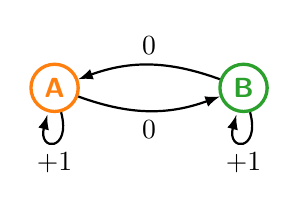
\begin{tikzpicture}
    \tikzstyle{n} = [very thick,circle,inner sep=0mm,minimum width=6mm]
    \tikzstyle{a} = [thick,>=latex,->]
    \def\dx{1.2}
    \def\dy{-1.2}
    \node[n,C1,draw=C1] (2) at (\dy,0) {\textbf{\textsf{A}}};
    \node[n,C2,draw=C2] (1) at (\dx,0) {\textbf{\textsf{B}}};
    \path[a]
    (2) edge [loop below] node {+1}(2)
    (1) edge [loop below] node {+1}(1)
    (2) edge [bend right=20] node[below] {0}(1)
    (1) edge [bend right=20] node[above] {0}(2);
\end{tikzpicture}

The reinforcement learning agent performs Q-learning.  Recall the $Q$ table has entries $Q(s,a)$. The $Q$ table is initialized with all zeros. The agent starts in state $s_1=A$. In any state $s_t$, the agent chooses the action $a_t$ according to a behavior policy $a_t = \pi_B(s_t)$. Upon experiencing the next state and reward $s_{t+1}, r_t$ the update is:
$$Q(s_t, a_t) \Leftarrow (1-\alpha) Q(s_t, a_t) + \alpha \left( r_t + \gamma \max_{a'} Q(s_{t+1}, a') \right).$$
Let the step size parameter $\alpha=0.5$.

\begin{enumerate}
\item (5 pts) Run Q-learning for 200 steps with a deterministic greedy behavior policy: at each state $s_t$ use the best action $a_t \in \argmax_a Q(s_t,a)$ indicated by the current Q table. If there is a tie, prefer move. Show the Q table at the end.

\item (5 pts) Reset and repeat the above, but with an $\epsilon$-greedy behavior policy: at each state $s_t$, with probability $1-\epsilon$ choose what the current Q table says is the best action: $\argmax_a Q(s_t,a)$; Break ties arbitrarily. Otherwise, (with probability $\epsilon$) uniformly chooses between move and stay (move or stay both with 1/2 probability). Use $\epsilon=0.5$.

\item (5 pts) Without doing simulation, use Bellman equation to derive the true Q table induced by the MDP.

\end{enumerate}

\end{document}
